
%(BEGIN_QUESTION)
% Copyright 2011, Tony R. Kuphaldt, released under the Creative Commons Attribution License (v 1.0)
% This means you may do almost anything with this work of mine, so long as you give me proper credit

This reversing motor control circuit has a problem: it runs just fine in reverse, but not at all in the forward direction.  A technician begins diagnosing the circuit, following the steps shown (in order):

$$\includegraphics[width=15.5cm]{i03532x01.eps}$$

\begin{itemize}
\item{} {\bf Test 1:} Jumpered points {\bf F} and {\bf G} while pressing the ``Forward'' pushbutton.  Motor did not turn.
\vskip 20pt
\item{} {\bf Test 2:} Measured 117 VAC between points {\bf G} and {\bf H} while pressing ``Forward'' pushbutton.
\vskip 20pt
\item{} {\bf Test 3:} Measured 478 VAC between points {\bf M} and {\bf N} while pressing ``Forward'' pushbutton.
\vskip 20pt
\item{} {\bf Test 4:} Measured 239 VAC between points {\bf M} and {\bf P} while pressing ``Forward'' pushbutton.
\vskip 20pt
\item{} {\bf Test 5:} Measured 239 VAC between points {\bf N} and {\bf P} while pressing ``Forward'' pushbutton.
\vskip 20pt
\medskip

Identify any useful information about the nature or location of the fault derived from the results of each test, in order of the tests performed.  If the test is not useful (i.e. provides no new information), mark it as such.  Assuming there is only one fault in the circuit, identify the location and nature of the fault as precisely as you can from the test results shown above.

\underbar{file i03532}
%(END_QUESTION)





%(BEGIN_ANSWER)

\begin{itemize}
\item{} {\bf Test 1:} Jumpered points {\bf F} and {\bf G} while pressing the ``Forward'' pushbutton.  Motor does not turn.  {\it While not a very efficient test, it does prove the problem is not an ``open'' M2 auxiliary contact.}
\vskip 5pt
\item{} {\bf Test 2:} Measured 117 VAC between points {\bf G} and {\bf H} while pressing ``Forward'' pushbutton.  {\it This proves the M1 coil is indeed receiving control power when it should.  Potential faults include an ``open'' M1 coil, or an ``open'' fault in the M1 power contacts.  This would have been a good \underbar{first} test!}
\vskip 5pt
\item{} {\bf Test 3:} Measured 478 VAC between points {\bf M} and {\bf N} while pressing ``Forward'' pushbutton.  {\it Proves at those two power contacts are closing as they should.}
\vskip 5pt
\item{} {\bf Test 4:} Measured 239 VAC between points {\bf M} and {\bf P} while pressing ``Forward'' pushbutton.  {\it Proves we do not have a good connection to line L3 through the third contact in the three-phase contactor.  The reduced voltage (239 volts versus 478 volts) is due to the motor's three-phase stator winding acting as a voltage divider, splitting the single-phase 478 VAC reading into two halves ($V_{MP}$ and $V_{NP}$).}
\vskip 5pt
\item{} {\bf Test 5:} Measured 239 VAC between points {\bf N} and {\bf P} while pressing ``Forward'' pushbutton.  {\it Proves again that we do not have a good connection to line L3 through the third contact.  Strictly speaking, this test is unnecessary.  However, since the conclusion drawn from Test 4 is not that obvious, this test would not be a bad idea simply to clarify the fact that the 478 VAC reading between M and N is being split in half.}
\end{itemize}

\vskip 10pt

{\bf The fault is an ``open'' between L and P (one of the power contacts within contactor M1).}

%(END_ANSWER)





%(BEGIN_NOTES)


%INDEX% Troubleshooting review: electric circuit diagnostic test rationale

%(END_NOTES)


